% Global
\documentclass[parskip=full,a4paper]{scrartcl}
\usepackage{blindtext}
\usepackage[utf8]{inputenc}
\usepackage{etoolbox}

% Graphics
\usepackage{pdfpages}
\usepackage{graphicx}
\usepackage{xcolor}
\usepackage[many]{tcolorbox}
\usepackage{etoolbox}

% Lists
\usepackage{enumitem}
\setlist{nosep} % or \setlist{noitemsep} to leave space around whole list

% Layout
\usepackage[margin=1in]{geometry}
\usepackage{setspace}
\usepackage[utf8]{inputenc}
\usepackage[english]{babel}
\setstretch{1.3}
% \setlength{\parindent}{0em}
% \setlength{\parskip}{1em}

% Inline-code
\usepackage[outputdir=./_build]{minted}
\definecolor{dhscodebg}{rgb}{0.01,0.199,0.1}
\setminted{
    fontsize=\scriptsize,
    baselinestretch=1.1,
    % bgcolor=dhscodebg,
    % rulecolor=\color{gray!40},
    % framesep=\fboxsep,
    % frame=single,
    % framesep=10pt
    % framerule=2pt,
    xleftmargin=2.5em,
    linenos,
    breaklines,
    tabsize=4
}
\usemintedstyle{tango}
\BeforeBeginEnvironment{minted}
{\begin{tcolorbox}[
            breakable,
            boxrule=0.2pt,
            colback=gray!40,
            % toprule=1pt,
            % rule=1pt,
            arc=0pt
        ]}\AfterEndEnvironment{minted}{\end{tcolorbox}}

% Bibliography
\usepackage{natbib}
\usepackage{bibentry}
\nobibliography*

% Title
\title{nETL}
\author{Zach Smith}
\date{\today}
\begin{document}


\section{nETL}
Many software packages exist to make analysis of such data trivial in terms of processing. Spreadsheet programs such as Microsoft Excel (or their online competition Google Sheets), databases such as Microsoft Access, MySQL are designed for this time of work.

But these tools fail when looking at scale of storage that Sakai's event data requires either in terms of ability (Microsoft Excel can work with a theoretical maximum of xxx lines, Access databases can be maximum 2GB), complexity or cost. Relational databases don't scale well horizontally speaking xxx, and this problem is going become more pronounced with time.

This thesis looks at creating a cost-effective 'analysis-engine' capable of scaling to many times the amount of data that a single machine can hold in a way that is still effective to analyze (distributed computing) and not too mentally taxing to implement.

specifically this project analyzed the viability of a software package called CouchDB, a NoSQL DBMS as a replacement for conventional RDMSs when analyzing data that has conventionally been housed RDBMSs (usually with an Oracle, Microsoft or SAP price tag associated with it).

\begin{figure}[h]
    \centering
    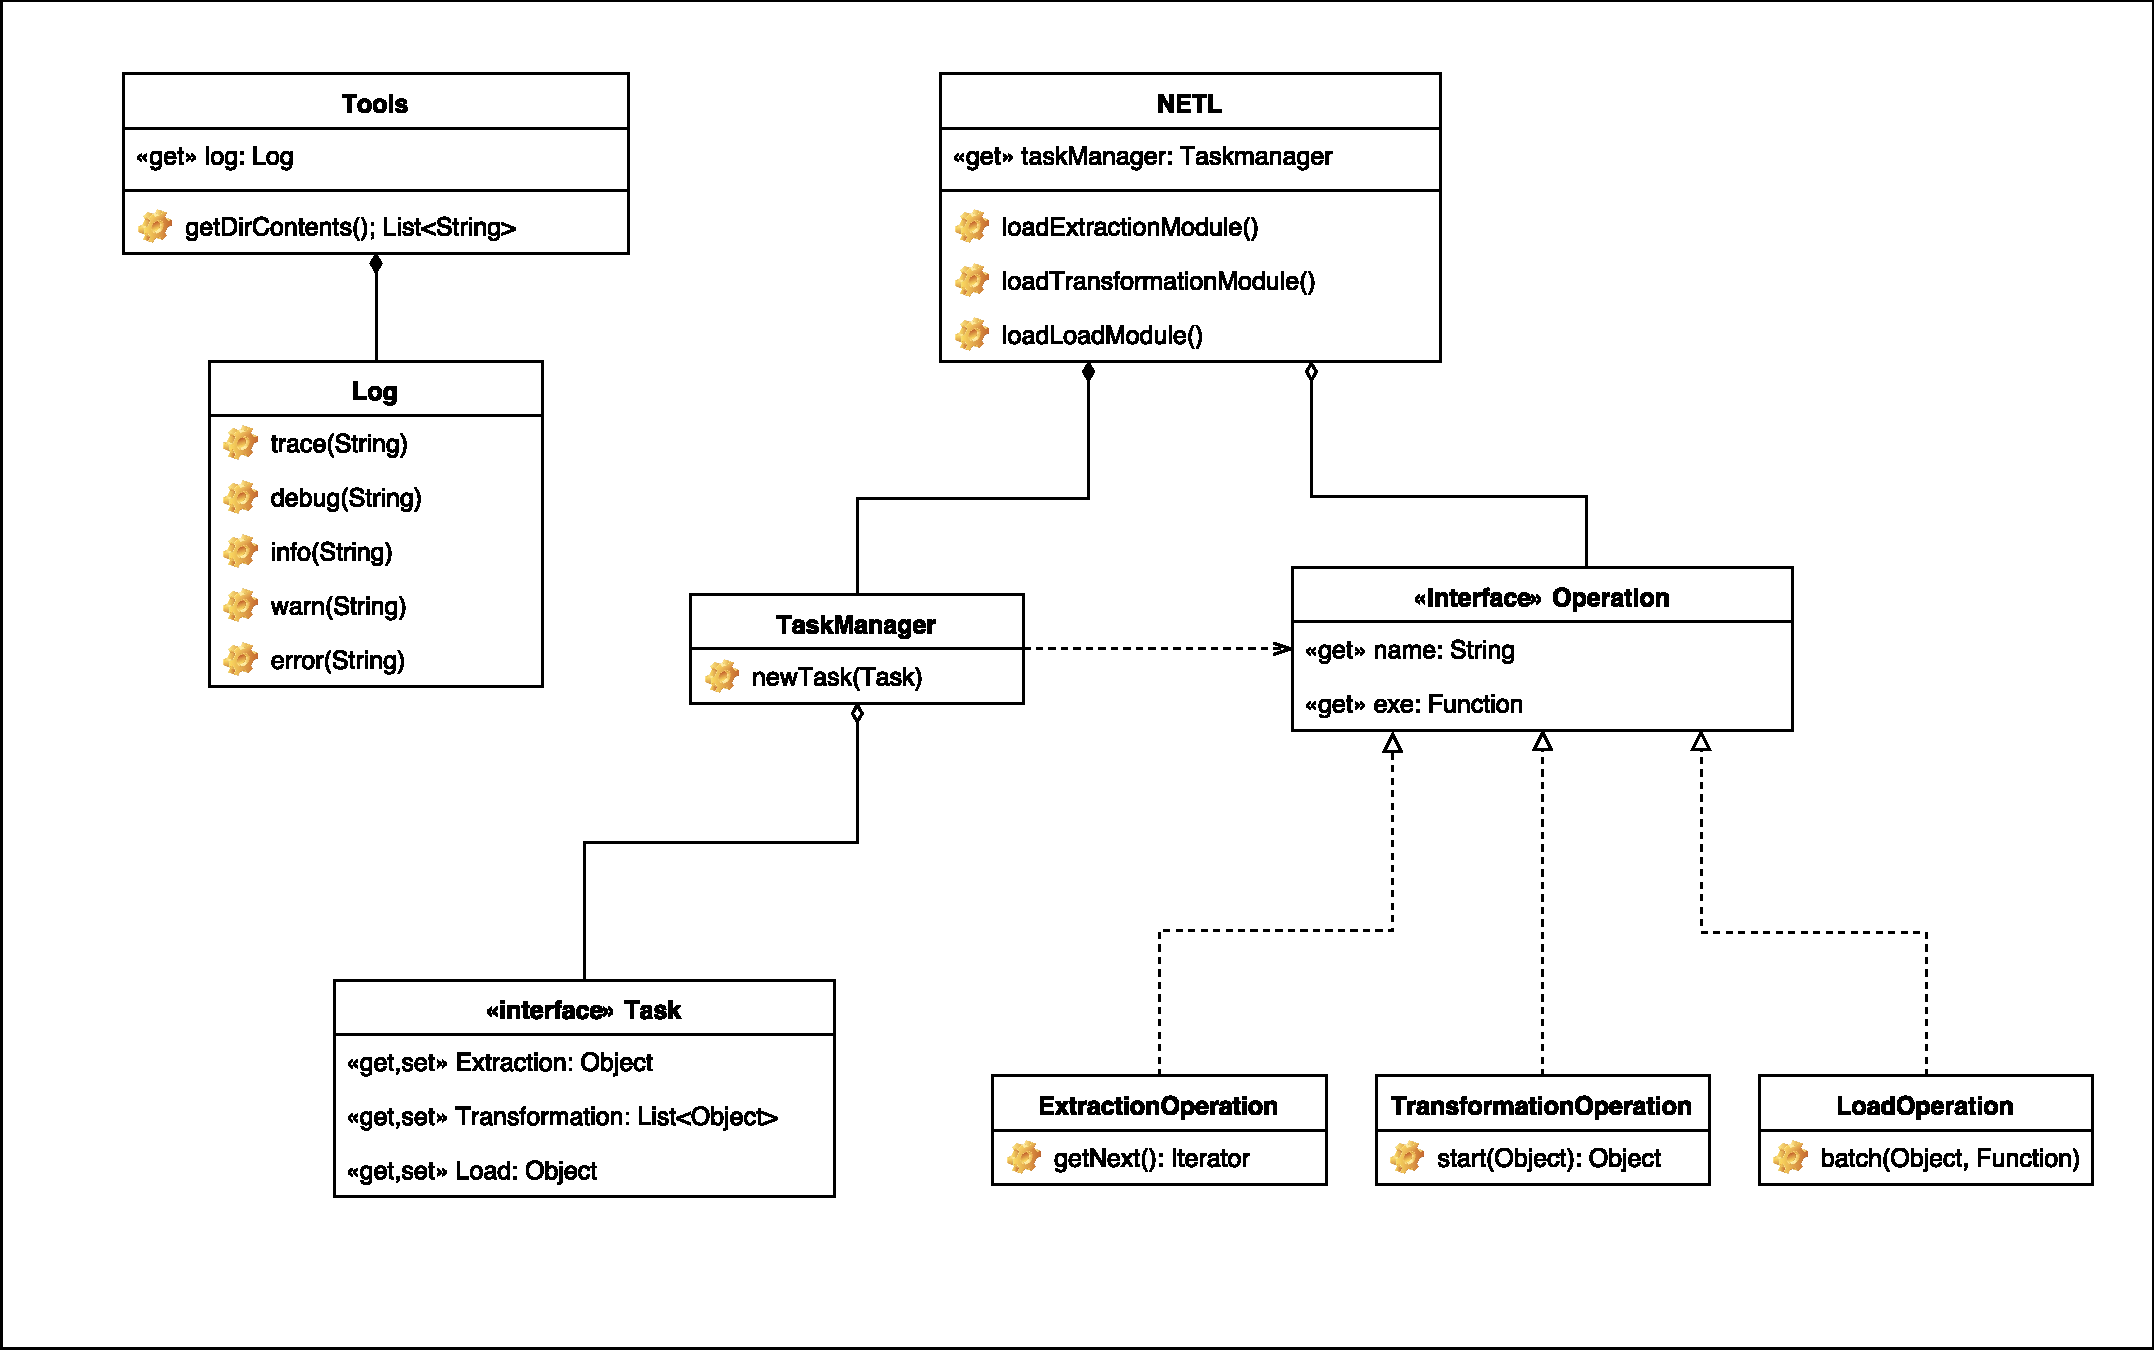
\includegraphics[scale=0.4]{../resources/figures/netlUML.pdf}
    \caption[nETL]{nETL}
    \label{nETL}
\end{figure}

Coming from a relational database environment there are a plethora of tools avaialable that facilitate transfer of CSV dato to a DBMS. These tools are available at a variety of different levels of extraction depending on a users technical skillset, time constraints and requirements. xxx: list some of these tools.

In a SQL Server environment SSDT (formerly SSIS) is considered the de facto standard for extracting/transforming and loading data between different data sources. xxx: find a graph on the usage of SSDT/SSIS in companies.

In fact it's likely that the availability of of SSDT/SSIS has influenced the uptake of SQL Server in operations that require dealing with large amount of data. It's fair to say that a barrier to using open source software such as CouchDB is the LACK of such software. Bespoke scripts are currently the only viable way of interfacing with CouchDB in a way that is comparable to SQL Server and SSDT. But with high-level languages such as node.js maturing, and the proliferation of small, focused libraries in these languages that abstract much of the unpleasant and gnarly aspects of bespoke scripting (xxx examples), bespoke data-scripting is nowhere near as difficult as it would be within the Microsoft environment (C\# or VB).

In line with the requirement of transferring large amounts of CSV data from a CSV source to CouchDB, and taking into account the comparatively low entry barrier to bespoke data-transformation scripts, a component of this MSc is an exploration of a possible alternative to SSDT for an environment other than Microsoft's SQL Server. This MSc project actually has several requirements that fall within the ETL spectrum that such a framework could easily be adapted to handle in a generic way. The framework has been published as an npm library and is available at ..., with source code available at github somewhere xxx.

Figure \ref{nETL} shows a potential architecture for a configurable component-based ETL tool. The intention of the framework is that it works on the basis of a pipeline of tasks. These tasks can be divided into 3 steps; an extraction step, a transformation step and a loading step. xxx insert something about ETL variations and why I chose the ETL pipeline.

\begin{enumerate}
    \item Extract data from a source specified by a user into memory
    \item Apply any number of transformations to the data in memory
    \item Load the data from memory into a destination specified by a user
\end{enumerate}

The framework itself is quite lightweight and comprises just the NETL, TaskManager and general purpose 'Tools' classes. For the purposes of this thesis, the framework as described by Figure \ref{nETL} has been prototyped in node.js with the source code available at xxx (there is also an npm package available at xxx). JavaScript is a suitable language to prototype this application for a number of reasons:

\begin{enumerate}
    \item It has a very succinct API making it fast to write code in (i.e. it is a highly abstracted language similarly to Ruby or Python)
    \item But unlike Ruby or Python (and other high level languages), it is opinionated in that it handles IO asynchronously by default
    \item The JavaScript implementation of object-orientation allows for easy runtime manipulation of the object model
    \item Another reason for choosing JavaScript is that it is very much in line with the spirit of CouchDB and the web in general
\end{enumerate}

\subsection{Implementation}

nETL is primarily a task-managing application, and as such, the TaskManager class is effectively the core of the application. It is intended that it can be instantiated as an instance (i.e. there can be many TaskManager instances hosted within a single running application). In JavaScript this is best implemented via a constructor:

\begin{minted}{javascript}
    /* File taskmanager.js */
    function TaskManager(extractions, transformations, loads) {
        this.tasks = {};

        // Hold references to extractions/transformation/loads of the main application process
        this.extractions = extractions;
        this.transformations = transformations;
        this.loads = loads;
    };

    TaskManager.prototype.newTask = function(task) {
        // Add task to this.tasks and execute the task
    };

    module.exports = TaskManager;
\end{minted}

The application itself is intended to be singleton instance of \mintinline{javascript}{class NETL{}}, which provides an IO interface (either a console terminal or otherwise) to TaskManager instances, and modular extraction/transformation and load operations. Singleton's are typically implemented via the modular pattern in JavaScript, which is typically how libraries are delivered to users by package managers and invoked by \mintinline{javascript}{var library = require('library-name')();}. One possible way of implementing the NETL class in JavaScript (i.e the method that is used within this project's code base) is shown here:

\begin{minted}{javascript}
    /* File netl.js */
    module.exports = function() {
        // Private properties / methods
        const _extractions = {};
        const _transformations = {};
        const _loads = {};        
        const _taskManager = new TaskManager(_extractions, _transformations, _loads);
        function _loadExtractionModule(extractionOperation){};
        function _loadTransformationModule(transformOperation){};
        function _loadLoadModule(loadOperation){};

        // Make process API available
        return {
            taskManager: _taskManager,
            loadExtractionModule: _loadExtractionModule,
            loadTransformationModule: _loadTransformationModule,
            loadLoadModule: _loadLoadModule
        };
    };
\end{minted}

And then the \mintinline{javascript}{NETL} singleton can be instantiated via the following code:

\begin{minted}{javascript}
    /* File <user entry point>.js */
    var NETL = require('./path/to/netl.js');
    var netl = NETL();
\end{minted}

% Close docuemnt
\end{document}